% Chapter 3
\chapter{Estado del Arte}
\label{Chapter3} % Change X to a consecutive number; for referencing this chapter elsewhere, use \ref{ChapterX}

En este Capítulo se encuentran trabajos anteriormente realizados que están relacionados con este proyecto, esto con la finalidad de presentar antecedentes, y dejar ver las discrepancias y similitudes existentes.\newline

El trabajo de dimensionar los sistemas de comunicación móviles es una necesitad recurrente en cada nueva generación celular. En \parencite{Celis2016}, se encuentra un proyecto terminal realizado por alumnos de la UPIITA, en el cual se realizó un simulador, bajo el paradigma de eventos discretos. El sistema objetivo era el celular 4G, con un enfoque en distintos esquemas de reúso de frecuencias y calendarizadores para obtener resultados sobre qué combinación de estos y bajo qué condiciones el sistema tenía un mayor desempeño. En este proyecto la simulación se llevó a cabo utilizando Matlab.\newline

Por otra parte, el reciente crecimiento de los casos de uso de IoT en una amplia gama de aplicaciones ha traído la necesidad de una mejor caracterización del tráfico tipo máquina. Reconociendo la importancia de esta cuestión, la 3GPP ha propuesto dos modelos para el tráfico tipo máquina. Se tratan de modelos de tráfico agregado . El primero modela el tráfico generado aleatorio, mientras que el segundo modela el tráfico síncrono con el tiempo. Dado que los modelos sólo se centran en el tráfico agregado, estos pueden no ser apropiados para el análisis práctico en algún sistema que esté más enfocado en el tráfico y requiera mayor precisión.\newline

En \parencite{Gupta2018}, los autores consideraron modelar el tráfico de dispositivos IoT conectados a través de tecnologías LPWAN. Debido a las diversas aplicaciones de IoT, no es trivial tener un solo modelo de tráfico para representarlas a todas, el tráfico puede clasificarse ampliamente como periódico, activado por eventos o una combinación de ambos. Evaluaron el rendimiento de LoRaWAN, en presencia de un híbrido de ambos tipos de tráfico, donde los eventos se propagan espacialmente a lo largo del tiempo. Utilizaron el modelo CMMPP para representar dicho tráfico característico de dispositivos IoT, que suelen ser activados por eventos.  \newline

De igual manera, pero ahora con un enfoque en sistemas celulares LTE, en \parencite{Smiljkovic2014} los autores analizaron el tráfico M2M con velocidad de datos variable bajo el supuesto de que la red LTE tiene recursos limitados. Los resultados muestran las características del tráfico M2M de una manera más realista, identificando las diferencias del tráfico estándar en la red celular. Revelan que el tráfico cuenta con la propiedad de auto similitud sólo para una gran cantidad de MTC.\newline

Estos trabajos muestran el uso de modelos de tráfico CMMPP para evaluar el impacto de la tecnología IoT. La integración del tráfico M2M será una parte inevitable de la evolución de las redes. En este proyecto se implementó el modelo CMMPP, en una red de 5G, teniendo en cuenta la arquitectura NB-IoT y distintas aplicaciones de IoT.\newline

Ahora bien, del lado de los esquemas de acceso no ortogonales (NOMA) en redes de quinta generación, se sigue trabajando en las propuestas de su implementación. En \parencite{Zhang2017}, los autores proponen un sistema usando geometría estocástica (PPP) para modelar un ambiente inalámbrico denso que admita NOMA tanto en el enlace de subida como en el enlace de bajada. \newline

En la implementación de NOMA propuesta, se tienen dos esquemas de emparejamiento de usuario: uno aleatorio y otro selectivo:
\begin{enumerate}
\item  Cuando el agrupamiento es aleatorio, los UE son seleccionados aleatoriamente.
\item  Cuando el agrupamiento es selectivo, el primer UE deberá tener una relación señal-interferencia más ruido (SINR) por encima del umbral T1 y el segundo UE tiene un SINR por debajo del umbral T2, T2 $\mathrm{\le}$ T1.
\end{enumerate}

Consideraron un error de propagación SIC durante el proceso de decodificación por parte del UE. Además, optaron por una estrategia de asignación de potencia fija, donde la potencia de enlace de bajada asignada a un UE está predefinida y permanece sin cambios.\newline

\begin{figure}
\centering
\begin{minipage}{.45\linewidth}
  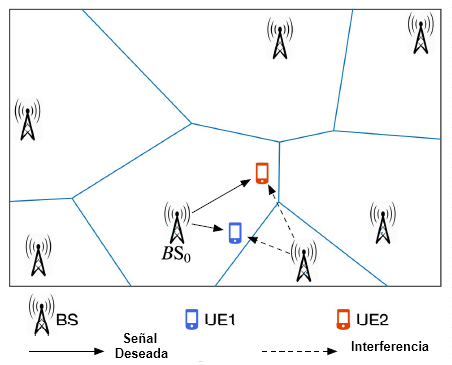
\includegraphics[width=\linewidth]{Modelo de sistema para el sistema de enlace descendente NOMA}
  \captionof{figure}{Modelo de sistema para el sistema de enlace descendente NOMA}
  \label{fig:img1}
\end{minipage}
\hspace{.05\linewidth}
\begin{minipage}{.45\linewidth}
  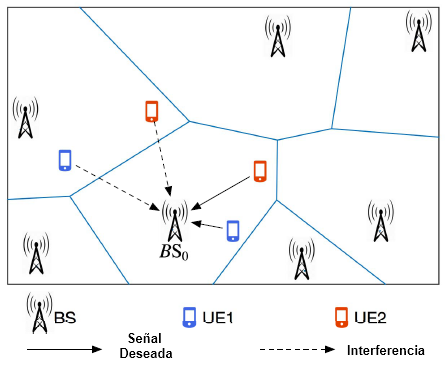
\includegraphics[width=\linewidth]{Modelo de sistema para el sistema de enlace ascendente NOMA}
  \captionof{figure}{Modelo de sistema para el sistema de enlace ascendente NOMA}
  \label{fig:img2}
\end{minipage}
\end{figure}

Las ganancias implementan el desvanecimiento de Rayleigh entre la $BS_0$ y $UE_i$. La ganancia en potencia de desvanecimiento Rayleigh entre BS y UE sigue una distribución exponencial con media 1 y se distribuye de forma independiente e idéntica (i.i.d.)\newline

En el enlace descendente (DL), agregaron perdidas por trayectoria con un exponente de pérdida y calcularon la interferencia entre celdas acumulativa de todas las bases adyacentes. En el enlace ascendente (UL), la interferencia inter-celdas proviene de todos los otros UEs que comparten la misma sub-banda. \textit{[Véanse Figuras~\ref{fig:img1}, \ref{fig:img2}]}\newline

Este trabajo se enfocó en realizar NOMA para sistemas 5G, sin embargo, no consideraron la actuación de dispositivos IoT, los cuales al tener diferentes calidades de servicio, impactarían en la toma de decisiones del modelo de acceso múltiple, más en concreto en el emparejamiento de usuarios.\newline

En \parencite{Mostafa2019} se trabajó en emplear NOMA para mejorar la densidad de conexión en los sistemas NB-IoT. En su propuesta cada subportadora puede dar servicio máximo a dos dispositivos con distintos requisitos de QoS. Formularon problemas de asignación de potencia de transmisión y subportadoras conjuntas para los modos singletone y multitone.  Además, propusieron algoritmos heurísticos con baja complejidad y dieron como resultado un rendimiento cercano a las soluciones óptimas y subóptimas en ambos casos. Los resultados de la simulación mostraron que el uso de NOMA aumentó la densidad de conexión hasta en un 87\% en comparación con OMA en el modo singletone y en el modo multitono, la densidad de conexión también se incrementó hasta en un 24\%.\newline

En \parencite{Shahini2019} desarrollaron un esquema NOMA en el dominio de potencia con agrupación de usuarios en un sistema NB-IoT. Resolvieron un problema de optimización para maximizar el rendimiento total de la red al optimizar la asignación de recursos de los dispositivos MTC y la agrupación de NOMA al tiempo que se satisfacen los requisitos de potencia de transmisión y QoS. Además, diseñaron un algoritmo heurístico eficiente para resolver el problema de optimización propuesto mediante la agrupación NOMA y la asignación de recursos a dispositivos de tipo máquina.\newline

En su modelo de sistema, consideraron el escenario de una única celda (eNB), que admite dispositivos de tipo máquina operando con la tecnología NB-IoT. Asumieron que no hay interferencia proveniente de otras células vecinas. \newline

\begin{figure}[th]
\centering
\includegraphics[scale=.6]{Figures/Modelo de sistema de una sola celda usando clusterización}
\decoRule
\caption[Grupos NOMA que incluyen dispositivos mMTC y URLLC, donde los dispositivos MTC comparten los subcanales asignados a cada clúster NOMA.]{Grupos NOMA que incluyen dispositivos mMTC y URLLC, donde los dispositivos MTC comparten los subcanales asignados a cada clúster NOMA.}
\label{fig:NOMA_NBIOT}
\end{figure}

Propusieron un esquema NOMA en el dominio de la potencia agrupando (de entre 1 a 4) dispositivos mMTC y URLLC en una red NB-IoT como se muestra en la Figura~\ref{fig:NOMA_NBIOT} . Según el esquema NOMA, los dispositivos mMTC y URLLC comparten cada subportadora (subcanal) y transmiten datos de manera no ortogonal. Por lo tanto, los dispositivos se dividen en diferentes grupos, llamados ``clusters''. Para decodificar con éxito los mensajes de la suma de mensajes recibida, el eNB emplea el esquema SIC. Por lo tanto, los usuarios deben ordenarse en cada grupo teniendo en cuenta el método SIC.\newline

Se ha investigado bastante acerca del desempeño de los esquemas NOMA para dispositivos IoT, sin embargo nuestra propuesta resulta diferente ya que además de utilizar PD-NOMA, se implementó un despliegue de UEs usando un PPP, un modelo de canal más realista y por último, un modelo de trafico de tipo fuente.
